\chapter{Webapp Description}

The features available on gTrack can be depicted using a flowchart presented in Figure 1. The features are discussed in details below.

Using bcrypt, we implemeted a secure user \textit{sign up} process that lets an interested visitor of the website become a registered user. Uniqueness of e-mail identification is ensured to prevent different users signing up with the same e-mail address.

Any user is able to see a detailed list of games that are present in Steam. The steam ID of a game is also recorded for easy viewing of the game in Steam. Various information associated with the game, such as cards, backgrounds, emotes, and price histories can also be viewed. As it is very common to look for games by genres or companies, two pages have been dedicated to summarize these information.

A registered user is allowed to \textit{comment} on games and \textit{like/dislike} games. However, any user can view previous comments made by other users on a game and also the total number of likes/dislikes associated with a game.

Registered users can access the in website chat room, \textit{gChat}, to communicate with other users.

Any user can \textit{search} for games based on various criteria, such as name, price range, company name, number of backgrounds/cards/emotes, average card/emote price, and system requirements.

\begin {figure}
\centering
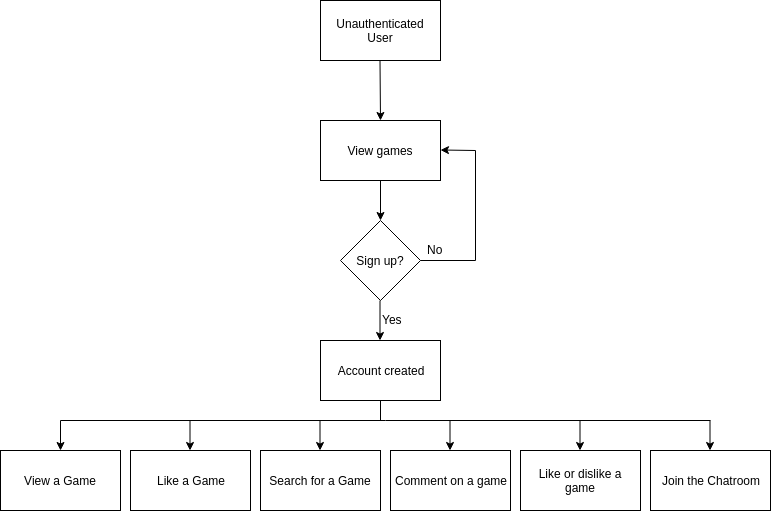
\includegraphics[width= 1\textwidth]{images/workflow.png}   
\caption{gTrack Flowchart}
\vspace{\floatsep}
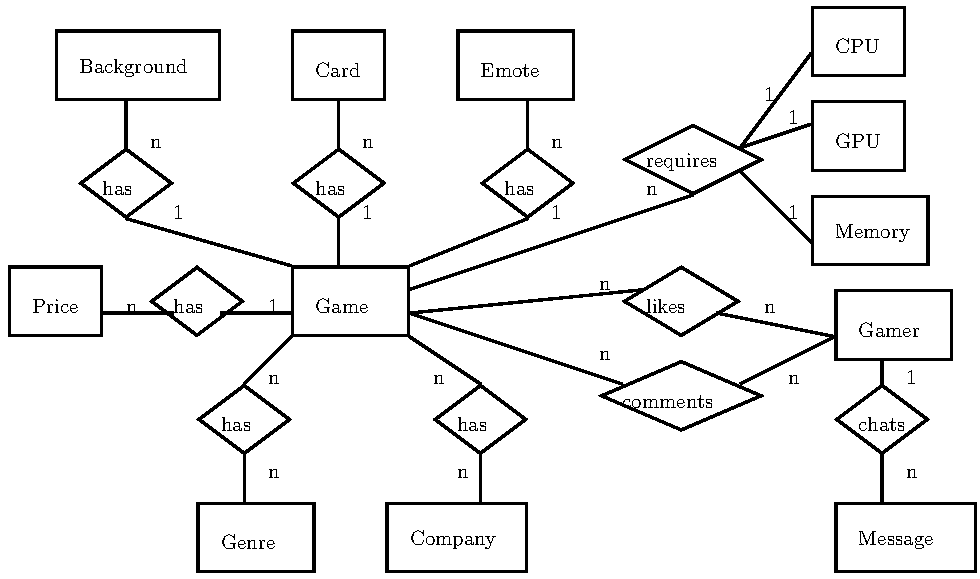
\includegraphics[width= 1\textwidth]{images/erd.pdf}   
\caption{Entity-relationship diagram.}\label{fig:erd}
\end{figure}

\section{Data Model}
As most modern applications tend to be highly data-driven, we made sure we had a sufficiently large dataset to work with. The entity-relationship diagram of our application has been presented in Figure~\ref{fig:erd}. We recorded information for 15453 games. There are 100 simulated users/gamers in our application, one being the admin. Each gamer can like/dislike a game and also comment on games. There are 775511 comments in total. Each game had price history associated with it. During seeding we used 436322 entries of price. The total number of backgrounds, cards, and emotes is 26066, 79133, and 33157. Apart from these, considerable amount of space was needed by the relations between games and genres/companies. The system requirements for each game was recorded too. The database contained ten types of processors, ten types of memories, and ten types of graphics cards. A few of the data fields in the seed file were synthetic, however, most of the data were collected through steam API to make the model resemble real data as closely as possible. Due to the sheer amount of seed data, we had to create our own SQL scripts instead of relying on ActiveRecords of Rails as the latter turned out to be too slow. The seed file alone was 361MB, whereas the size of the database after seeding was 389MB.
